\documentclass[main]{subfiles}

\begin{document}
\chapter{Marco Referencial}

	Este capítulo provee la evolucíon historica del estudio del fenómeno de deslizamiento en el contacto mecánico entre las superficies de la rueda y el riel bajo rodadura que permitió interpretar los resultados obtenidos de este trabajo. Así mismo, describe los antecedentes del problema en el contexto de las investigaciones realizadas en los tópicos del contacto mecánico y la rugosidad, y los trabajos realizados en la compañía Metro de Caracas C.A.

\section{Antecedentes de la investigación}

	 El conocimiento del contacto mecánico rueda-riel y de la rugosidad de las superficies desarrollados  por \citet{Kalker1982VSD} y \citet{Greenwood06121966} se engloban dentro de los parámetros del contacto mecánico, sin embargo presentan condiciones distintas: el contacto rueda-riel estudia los esfuerzos provocados por el contacto entre las superficies, con magnitudes que rozan la barrera elástico-plástico, mientras que la rugosidad es estudiada por sus efectos vibratorios y de ruido a causa de las irregularidades de la superficie.
	 
	 Los antecedentes de este proyecto se constituyen en la investigación realizada por Metro de Caracas C.A. sobre el comportamiento en la dinámica ferroviaria en la linea 1 y los artículos que refieren a las irregularidades en la superficie de los cuerpos y sobre el fenómeno de deslizamiento en vigas curvas, además del desarrollo continuo al algoritmo de \citet{Kalker1982VSD}, FASTSIM.

\subsection{Trabajos realizados por la empresa Metro de Caracas}

	En el año 1999, la compañía Metro de Caracas C.A. realizó investigaciones para determinar las condiciones del comportamiento dinámico del sistema ferroviario con la finalidad  de mejorar las condiciones del servició tanto en el ámbito estructural como en el confort para los usuarios.

	Para la investigación realizada por Metro de Caracas se solicitó el asesoramiento de la Corporación del Centro Tecnológico de Transporte (Transportation Technology Center, Inc. o sus siglas en ingles TTCI). Mediante un convenio, que no solo implicaba la contratación de los servicios de TTCI para la realización de pruebas experimentales, sino que también se incluyo la transferencia tecnológica mediante la compra de la instrumentación utilizada en las pruebas.

	Las pruebas realizadas por TTCI, consistieron en la evaluación de la dinámica del bogie y de los componentes motrices del que está compuesto (motor, caja de engranajes, chasis) y la dinámica del vagón y el tiempo estimado de vida del bogie sometido a cargas alternantes. Para este trabajo se realizó con mayor énfasis una investigación bibliográfica sobre las actividades llevadas acabo en el estudio de la dinámica bogie-vagón donde se recogieron datos sobre la dinámica del contacto rueda-riel.
	
	Durante las pruebas ferroviarias se utilizó una serie de instrumentos de medición conformados por acelerómetros, manómetros y sensores de posición para interpretar el comportamiento vibratorio de los distintos componentes del bogie. Adicionalmente se incorporó a la instrumentación, un bogie de Metro de Caracas C.A. cuyas ruedas fueron modificadas con un juegos de galgas extensiométricas para la detección de las cargas verticales, laterales y longitudinales en la superficie de la rueda, adicionalmente se incluyó una serie de galgas para la determinación de la posición de en la que se encuentra el punto de contacto.
	
	Pese a que el uso de ejes instrumentados fue utilizado principalmente para la evaluación del comportamiento vibratorio de los componentes motrices y del bogie, la metodología implementada por TTCI, fue comparando los resultados obtenidos con una simulación computarizada mediante el software NUCARS (software creado por la TTCI para la simulación de la dinámica multicuerpo de vehículos). NUCARS, incluye dentro de sus rutinas de operación, la simulación del contacto rueda riel para las cargas laterales, longitudinales de acuerdo al comportamiento del eje.
	
	En los informes finales de TTCI, no se hace mención de observaciones realizadas sobre el comportamiento del deslizamiento en la superficie de la rueda. No obstante TTCI dejo una serie de datos bibliográficos sobre el uso, construcción y la logística emprendida por la empresa para la recolección de datos, además de los mismos datos obtenidos en pruebas en vía que fueron utilizados para la elaboración del instrumento.

\subsection{Rugosidad} 

  En lo que respecta a la rugosidad, las diferencias en el modelo de \citet{Herz1881} referente al área real de contacto, fueron observadas por \citet{Bowden07021939} al establecer una relación entre el área de contacto y la conductancia de la zona de contacto. La estimación del área real de contacto se obtuvo de manera estadística y fue descrita por \citet{Greenwood06121966}, en función de la irregularidades de la superficie.
  
La rugosidad o las irregularidades en la superficie han cobrado importancia en el estudio de la sensibilidad de distintos componentes electrónicos que han sido miniaturizados. Una recopilación de métodos para describir las irregularidades en la superficie fue planteado por \citet{Patrikar2004213}, utilizando los valores estadísticos prácticos que se obtienen al estudiar una superficie rugosa.
  
\citet{Patrikar2004213} se enfoca en cuatro métodos para simular la rugosidad: el método de la transformación rápida de Fourier, la función de Mandelbrot–Weierstrass, mediante redes neurales artificiales y por último el método de propagación inversa. Estos métodos se utilizaron para la generación de fractales y describir las irregularidades de una superficie. 

El método de la transformación de Fourier rápida, puede simular la altura de una superficie en un punto de coordenadas (x,y) mediante la siguiente ecuación:


\begin{equation}
f(x,y)=\sum_{k=0}^{M-1}\sum_{l=0}^{N-1}\sqrt{S_{k,l}}
\cdot e^{\left( i2\pi \left[ 
\phi_{k,l}+\frac{kx}{M}+\frac{ly}{N}
\right[ \right)}
\end{equation}

\par \hspace{1cm}
\begin{minipage}{10cm}
\begin{spacing}{0.5}
Donde:
\begin{itemize}
\item $S_{k,l}$ es la densidad espectral de la rugosidad
\item $R_rms$ la desviación estándar de las irregularidades:
\end{itemize}
\end{spacing}
\end{minipage}


\begin{equation}
S_{k,l}=\frac{1}{MN}\sum_{k=0}^{M-1}\sum_{s=0}^{N-1} R_{rms}
\cdot e^{\left( -i2\pi \left[ 
\frac{kr}{M}+\frac{ls}{N}
\right[ \right)}
\end{equation}

Otro método es la generación de fractales propuesto por Mandelbrot–Weierstrass donde la altura de las irregularidades viene dado por:

 \begin{equation}
f(x)=\sum_{n=-\infty}^{\infty} b^{-n(2-D)} [1-k\cos(b^nx+\phi)]
\end{equation}
  
  \par \hspace{1cm}
\begin{minipage}{10cm}
\begin{spacing}{0.5}
  Donde 
\begin{itemize}
\item $b$ es el múltiplo de la frecuencia que ronda entre 1.1 y 3.0.
\item $D$ es la dimensión fractal que varia entre 1 y 2 viene dado por $D=\frac{\ln(N)}{\ln(1/r)}$.
\item  $\phi$ es la fase incial, y es un numero aleatorio entre 0 a 2$\pi$.
\item $k$ es un valor utilizado para afectar el resultado aunque usualmente viene dado por 1.
\item Para obtener la mejor simulación, se modifica los valores D, k y b hasta alcanzar el una superficie cuya desviación estándar se aproxime a $R_rms$.
\end{itemize}  

  \end{spacing}
\end{minipage}
  

	El trabajo de \citet{Patrikar2004213} fue enfocado en las propiedades eléctricas de los condensadores eléctricos, que motivado a su miniaturización, han aumentado su sensibilidad a sufrir cambios en la capacitancia del dispositivo por las irregularidades presentes en la superficie. Por tanto la conclusión alcanzada por el autor, donde se establece que los métodos de redes neurales poseen una mejor aproximación a la geometría de la superficie, son enfocadas al comportamiento eléctrico y no al comportamiento mecánico.
	
	La investigacion sobre el modelado de superficies rugosas elaborada por \citet{Patrikar2004213} es tomada en cuenta en este trabajo para establecer el nivel evolutivo que ha alcanzado el estudio de las singularidades en la superficie. El grado de precisión necesaria para considerar su uso en el estudio de capacitancia eléctrica en dispositivo miniaturizados ha de ser elevado por lo que su uso para definir superficies rugosas puede resultar útil cuando requiere un alto grado de exactitud.
	
	 En referencia al grado de precisión de las redes neurales inversas, para fines del comportamiento mecánico el grado de precisión se aprecia a una escala mayor de la que se puede esperar en condensadores miniaturizados. Motivado a esto, el modelo de \citet{Greenwood06121966} permite un modelado efectivo de la interpretación que se tiene sobre la rugosidad en una superficie y sus efectos en el contacto mecánico rueda riel.
	 
	 En el ámbito del contacto mecánico, los aportes de \citet{Patrikar2004213} no forman parte de este tema. Sin embargo, \citet{Kalker1990} realizó un modelado de interacción rueda-riel bajo conceptos similares.
  
  
\subsection{Contacto Rueda-Riel}  
  
	Sobre la dinámica de los sistemas ferroviarios, existen numerosos algoritmos para el cálculo de las cargas tangenciales \citet{Kalker1991243}. El más utilizado comercialmente es la teoría lineal del contacto rueda-riel, propuesta por \citet{Kalker1971VSD}, luego el modelo de Shen-Hedrick-Elkins para deslizamientos no lineales mencionado por \citet{Kalker1991243} y \citet{springerlink:10.1007/s11044-007-9094-y} y el modelo de \citet{Polach1999}.

Para la simulación del contacto rueda riel, es necesario conocer con precisión el punto de contacto, el cual resulta complejo debido al perfil geométrico de la rueda y el riel y al movimiento propio de los componentes del vehículo. Es por ello, que fue necesario establecer un modelo para determinar el punto de contacto introduciendo los parámetros geométricos de la vía, además el modelo predice cuando existen dos puntos de contactos simultáneos en una misma rueda. Este modelo fue definido por \citet{springerlink:10.1007/s11044-007-9094-y}. La metodología  consistió en la parametrización geométrica de las vías como se muestra en el esquema de la figura \ref{fig:Pombopar}, la determinación del punto de contacto como se representa en la figura \ref{fig:Pombopar2}, y el estado del contacto mecánico en el punto seleccionado.

	Las conclusiones obtenidas por \citet{springerlink:10.1007/s11044-007-9094-y} establecen que ante grandes curvaturas, el modelo de Kalker no es viable debido a que las cargas tangenciales se aproximan al límite de la fricción propuesto por en Coloumb. 

	El modelo de Shen-Hedrick-Elkins da resultados pocos precisos cuando existen cambios de concavidad en puntos del rueda cuya geometría posee grandes diferencias. Dejando el modelo de \citet{Polach1999} como el modelo que mejor aceptación tiene con bajos radios de curvatura \citet{springerlink:10.1007/s11044-007-9094-y}.

\begin{figure}[!htbp]
\centering
    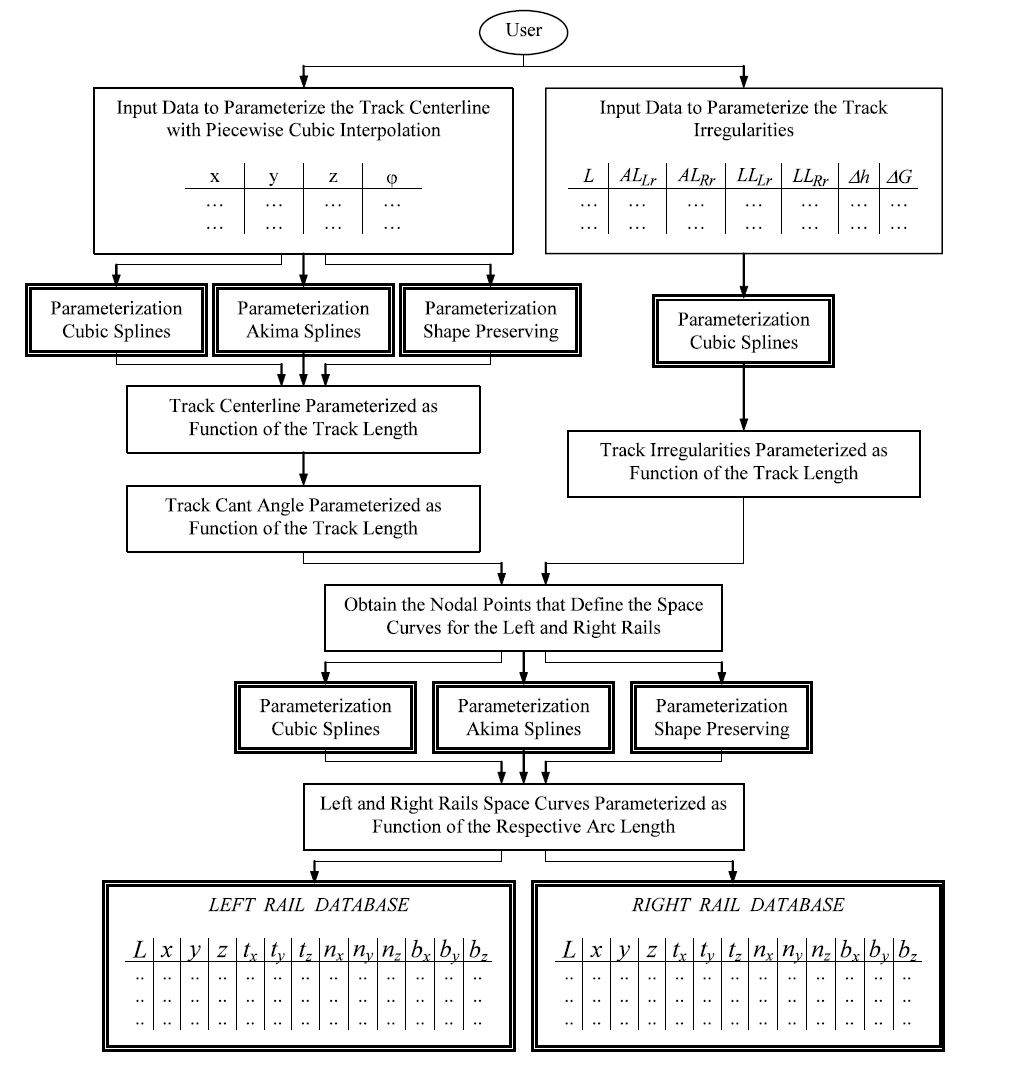
\includegraphics[scale=0.4]{Pombopar.png}
  \caption{Esquema que representa la parametrización  de la geometría del riel, \citet{springerlink:10.1007/s11044-007-9094-y}. Donde el usuario incorpora datos geometricos tanto de la rueda como el riel, para que estos sean parametrizados y utilizados en los algoritmos de Kalker, Shen et al y Polanch.}
  \label{fig:Pombopar}
\end{figure}  
\newpage

\begin{figure}[!htbp]
\centering
    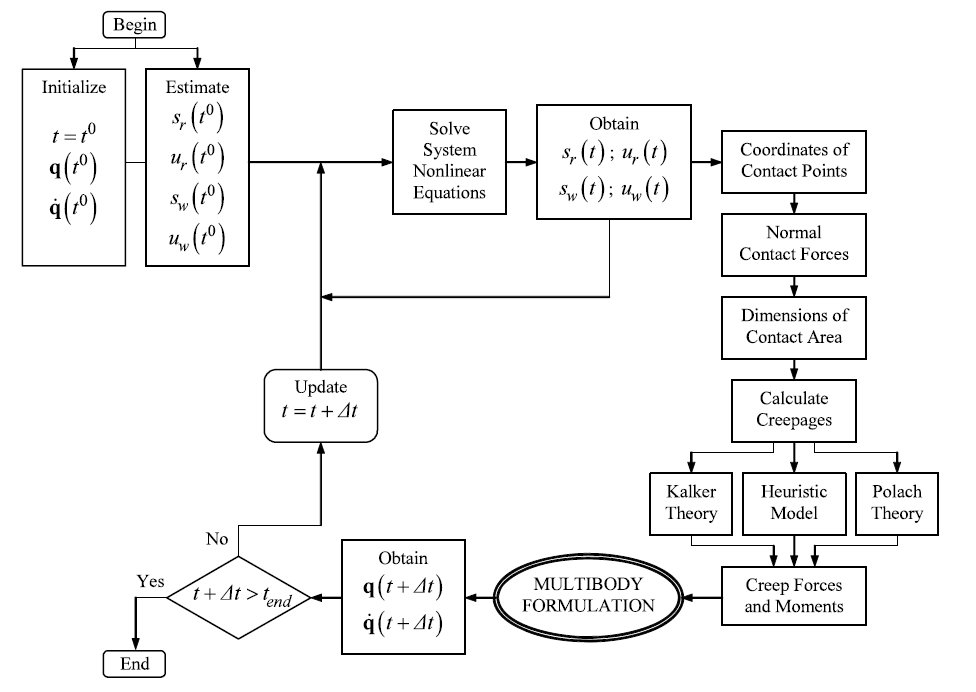
\includegraphics[scale=0.3]{Pombopar2.png}
  \caption{Esquema que indica el procedimiento de contacto mecánico rueda-riel, \citet{springerlink:10.1007/s11044-007-9094-y}. Este modelo tiene mayor afinidad a la parametrización de las distintas configuraciones dispuestas en la interacción rueda-riel.}
  \label{fig:Pombopar2}
\end{figure}  

	Pese a las conclusiones de \citet{springerlink:10.1007/s11044-007-9094-y}, el modelo Kalker es efectivo para tramos longitudinales o de curvaturas suaves, siendo óptimo para trenes de alta velocidad o cuya geometría así lo sugiere. En este caso \citet{2011CompM..47..105V} continúan las investigaciones de \citet{Kalker1971VSD} para obtener una respuesta al problema de contacto mecánico con mayor aproximación a los valores teóricos.

	La base del algoritmo de Kalker en FASTSIM utiliza metodos de primer orden para soluciónar ecuaciones diferenciales y determinar el comportamiento del contacto mecánico a cargas tangenciales dentro de la zona de adhesión. Vollebreght (2010) propone un algoritmo distinto utilizando métodos de segundo orden, al cual denomina ''FASTSIM2''.

	El contacto rueda riel, dado por las cargas tangenciales, se centra principalmente en distinguir el deslizamiento rígido del deslizamiento elástico. Esta interacción se hace presente en la dinámica provocada por el roce, tal como es mencionada por Coulomb: directamente proporcional a la compresión que se aplica en la superficie. Considerando que el modelo de Hertz establece el perfil de presiones normales, se puede obtener entonces los limites de las cargas tangenciales dentro del rango de adhesión denominado domo de saturación.
  
El principio de Kalker se define por la deformación normal de la superficie en la dirección de traslación; la diferencia entre el deslizamiento rígido $s(x)$ y el deslizamiento elástico $w(x)$ es por tanto la deformación normal $\frac{du_x}{dx}$, tal como se define en la ecuación (\ref{Kalker1}):

\begin{equation}
\label{Kalker1}
\frac{du_x}{dx}=s(x)-w(x)
\end{equation}

\par \hspace{1cm}
\begin{minipage}{10cm}
\begin{spacing}{0.5}
Donde:
\begin{itemize}
\item $u_x$ es el desplazamiento de partículas en la dirección de la traslación de la rueda.
\item $s(x)$ el deslizamiento elástico.
\item $w(x)$ el deslizamiento rígido.
\end{itemize}
\end{spacing}
\end{minipage}

El método de Euler original propuesto por Kalker, define con gran precisión el deslizamiento elástico, sin embargo la definición del área de adhesión no es del todo precisa segun lo define \citet{2011CompM..47..105V} y tiene cierto grado de error como se observa en la figura \ref{fig:KalkervsFastsim2} donde se muestra la diferencia entre los resultados obtenidos por el método de Euler y un método trapezoidal para solucionar la ecuación diferencial de contacto rueda-riel \ref{Kalker1}.

\begin{figure}[!htbp]
\centering
    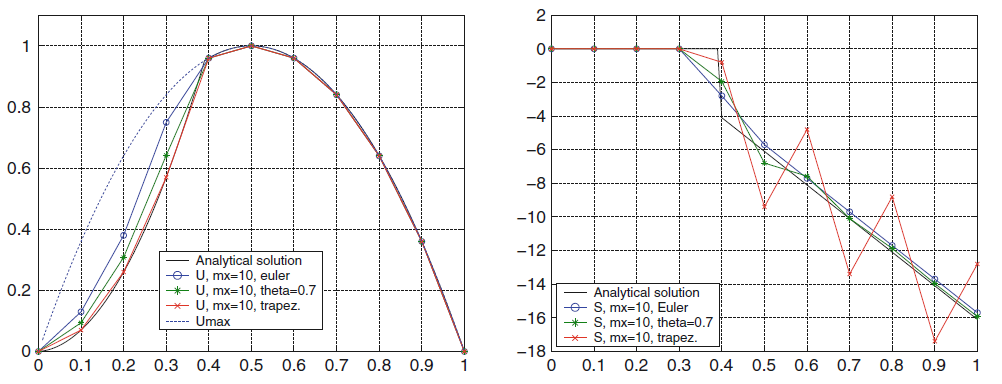
\includegraphics[scale=0.55]{Kalker1.png}
  \caption{Diferencias entre el método de euler, método analítico y método trapezoidal.}
  \label{fig:KalkervsFastsim2}
\end{figure}  

\pagebreak 

FASTSIM2 sigue el siguiente algoritmo para resolver la ecuación diferencial (\ref{Kalker1}).


\begin{equation}
\label{FastSim21}
u_i=u_{i-1}+\frac{\delta x}{2}(s_i+s_{i-1})-\frac{\delta x}{2}(w_i+w_{i-1})
\end{equation}

\begin{equation}
\label{FastSim22}
\tau_i=L^{-1}u_i
\end{equation}

\par \hspace{1cm}
\begin{minipage}{10cm}
\begin{spacing}{0.5}
\begin{itemize}
\item $u_0=0$ y $\tau_0=0$, se estima $s_0=(||w_0||-L\mu p_{n_{i}})\frac{w_0}{||w_0||}$ si es necesario.
\item Para cada valor $x_i$ se calcula previamente $u_i^{adh}$ y $\tau_i^{adh}$  considerando $s_i=0$.
\item Si $||\tau_i^{adh}||<\mu p_n$ entonces se confirma que $s_i=0$ y por lo tanto $u_i^{adh}=u_i$ y $\tau_i^{adh}=\tau_i$.
\item Si $||\tau_i^{adh}||>\mu p_n$ se estima que 
$\tau_i=\mu p_n \frac{\tau_i^{adh}}{||\tau_i^{adh}||}$ por lo tanto $u_i=L \tau_i$ mientras que el deslizamiento elástico $s_i=2\frac{u_i-u_i^{adh}}{\delta x}$ .
\end{itemize}
\end{spacing}
\end{minipage}

El resultado de este algoritmo es la capacidad de poder estudiar el contacto mecánico con una matriz de 10 x 10 con resultados definidos por Vollebregt (2011). FASTSIM2 es la ultima investigacion realizada con base a los trabajos de Kalker para simular el contacto rueda-riel.

\subsection{Contacto rueda-riel y las irregularidades en la superfice de contacto.}

Ultimo trabajo de Kalker

RAILCCS

\section{Fundamentos teóricos}

En la teoría de la elasticidad de los materiales, las deformaciones son producto de la interacción de fuerzas con el cuerpo, tanto en su superficie como dentro de su volumen. Así lo define Hertz (1881) para introducir la mecánica de contacto al estudio de la teoría de cuerpos elásticos.

\subsection{Contacto mecánico hertziano}

 El modelo de Hertz tuvo dos objetivos: determinar una distribución de presión que se aproximara al contacto real entre ambas superficies y el dimensionamiento de esta distribución. Para cumplir estos objetivos, Hertz modela las superficies de contacto en función de las curvaturas y la profundidad de las mismas, como se observa en la figura \ref{fig:PlotZAB}:
  
\begin{figure}[!htbp]
\centering
    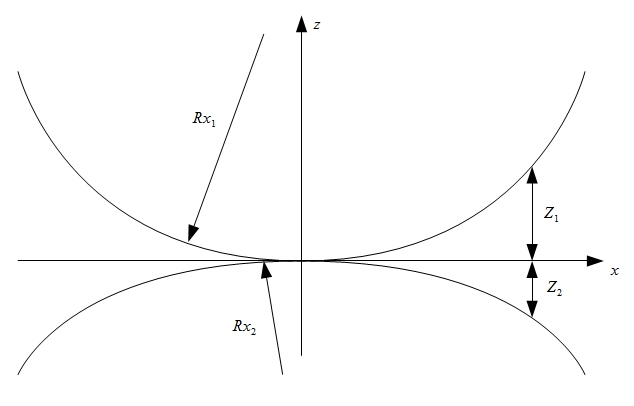
\includegraphics[scale=0.7]{FigZZ.png}
  \caption{Superficies con curvatura donde el contacto se inicia en el centro de coordenadas.}
  \label{fig:PlotZAB}
\end{figure}  
  
Estas superficies pueden ser descritas considerando los radios de curvatura $R_x$ y $R_y$ de cada cuerpo $i=1,2$:

\begin{equation}
A_i=\frac{1}{2R_{xi}} \: B_i=\frac{1}{2R_{yi}}
\end{equation}

Por lo tanto se puede describir analíticamente una superficie en coordenadas x,y como:

\begin{equation}
Z_i=A_ix^2+B_ix^2
\end{equation}

De modo que la distancia entre dos puntos cuando el contacto entre las dos superficies se da en un punto z=0

  \begin{equation}
  Z_1-Z_2=Ax^2-By^2
  \end{equation}

\par \hspace{1cm}
\begin{minipage}{10cm}
\begin{spacing}{0.5}
Donde:
\begin{itemize}
\item A y B son constantes basadas en las curvaturas de ambas superficies $A=\frac{1}{R_x1}+\frac{1}{R_x2}$ y $B=\frac{1}{R_y1}+\frac{1}{R_y2}$.
\item $Z_1$ y $Z_2$ la profundidad de penetración entre el plano de contacto
\end{itemize}
\end{spacing}
\end{minipage}

 Al tratarse de dos cuerpos elásticos, la elasticidad de ambas superficies permite una deformación normal al plano de contacto, de modo que ambas superficies forman una superficie plana de contacto:

\begin{figure}[!htbp]
\centering
    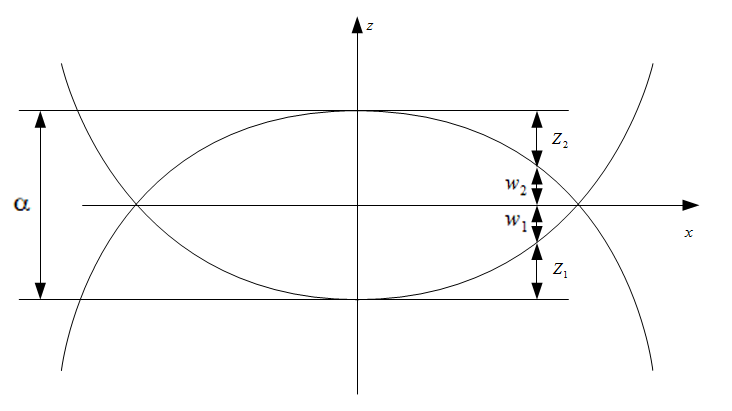
\includegraphics[scale=0.7]{FigZwalpha.png}
  \caption{Superficies interceptadas, donde el plano de contacto es representado por $z=0$ y el desplazamiento de un punto respecto a la dirección normal $w_1$ y $w_2$.}
  \label{fig:PlotZww}
\end{figure} 

La distancia entre los puntos de máxima curvatura $\alpha$ viene dado por:  

  \begin{equation}
  \label{eq:Eq2}
  Z_1-Z_2+w_1+w_2=\alpha
  \end{equation}

\par \hspace{1cm}
\begin{minipage}{10cm}
\begin{spacing}{0.5}
Donde:
\begin{itemize}
\item $w_1$ y $w_2$ corresponden a las compresiones en un determinado punto en las coordenadas (x,y).
\item $\alpha$ la deformación normal máxima en el centro de coordenadas (x,y).
\end{itemize}
\end{spacing}
\end{minipage}

Tal como se visualiza en la figura \ref{fig:PlotZww}, $\alpha$ es la deformación máxima en la dirección normal, $w_1$ y $w_2$ la deformación a lo largo del eje z en un punto de coordenadas (x,y). 

La solución planteada por Lamor (1892) para el desplazamiento de partículas en una superficie es mencionada por \citet{timoshenko1970theory}. En ella, cuando se aplica una carga puntual P sobre un plano cuyo espacio inferior es elástico, se puede definir como:

  \begin{equation}
  \label{eq:Eq3}
  w=\frac{P \cdot (1-\nu^2)}{\pi \cdot E \cdot r}
  \end{equation}

\par \hspace{1cm}
\begin{minipage}{10cm}
\begin{spacing}{0.5}
Donde:
\begin{itemize}
\item $w$ el desplazamiento de un punto en la superficie.
\item $P$ es una carga puntual aplicada en determinado punto.
\item $\nu$ el módulo de Poisson.
\item $E$ es módulo de Young.
\item $r$ la distancia entre el punto de aplicación de la fuerza con un punto de estudio cualquiera.
\end{itemize}
\end{spacing}
\end{minipage}

Al evaluar el desplazamiento de una partícula ubicada en el centro de aplicación de la carga en una superficie ($r=0$), tanto los esfuerzos como los desplazamiento son infinitos. Se puede evitar esta discontinuidad, considerando $P$ como una carga distribuida a lo largo de un radio pequeño $r$ de modo que el término $\frac{P}{r}$ se reduce a $q$ como la distribución radial de cargas, tal como lo expresa \citet{timoshenko1970theory}. Esta interpretación permite expresar el desplazamiento normal de una particula ($w$) para el contacto mecánico como:

\begin{equation}
\label{eq:Eq4}
w=\frac{(1-\nu^2)}{\pi \cdot E}  \iint\limits_{A} q ds d\psi
\end{equation}


Para simplificar el desplazamiento de una particula expresada en forma integral (\ref{eq:Eq4}) se plantea una constante de compresión que viene dada por:

\begin{equation}
k=\frac{(1-\nu^2)}{\pi \cdot E}
\end{equation}
  
  La forma analítica de intersección entre dos superficies (\ref{eq:Eq2}) puede ser expresada como la suma de las integrales de el desplazamiento normal de una particula ($w$) en función del desplazamiento de partículas en la dirección normal (\ref{eq:Eq4}) obteniendo:
  
  \begin{equation}
  \label{eq:Eq5}
  \left(
  k_1+k_2
  \right)
  \iint q ds d\psi =\alpha-Ax^2-By^2
  \end{equation}

Para poder resolver la integral del desplazamiento de particulas en la superficie (\ref{eq:Eq5}) se estudia el contacto para superficies cuyas curvaturas son proporcionales ($Rx_1=Ry_1$ y $Rx_2=Ry_2$) entre si, permitiendo definir la geometría de las superficies en coordenadas cilíndricas, de modo que $A=B=\beta$ y se plantea la forma analítica de los cuerpos interceptados (\ref{eq:Eq5}) en coordenadas cilíndricas.

  \begin{equation}
  \label{eq:Eq51}
  \left(
  k_1+k_2
  \right)
  \iint q ds d\psi =\alpha-\beta r^2
  \end{equation}
  
  Para la distribución de cargas $q$ que satisfaga la integral de los desplazamiento en la dirección normal (\ref{eq:Eq51}) se puede establecer que la presión máxima es proporcional al radio máximo de la superficie de contacto, $k=q_o/R_{max}$ donde $q_o$ es la presión máxima y $R_{max}$ el radio máximo de zona de contacto. Obteniendo una solución para la primera integral de los desplazamientos de las partículas en la superficie.

\begin{equation}
\label{eq:SolvInt}
\int qds=\frac{q_o}{R_{max}}\cdot U
\end{equation}

Donde $U$ es el área de un perfil de presión propuesto en el plano de coordenadas $(z,r)$, si se considera que el perfil de presión es una semiesfera de radio $R_{max}$, se obtiene que el desplazamiento de partículas en coordenadas cilíndricas (\ref{eq:Eq51}) se replantea del siguiente modo:

 
   \begin{equation}
  \label{eq:Eq6}
    \left(
  k_1+k_2
  \right)
  \int \frac{q_o}{a}\cdot \pi(R_{max}^2-r^2\cdot \sin ^2(\psi)) d\psi =\alpha-\beta r^2
  \end{equation}
 
 La solución de la ecuación (\ref{eq:Eq6}) es finalmente:
 
  \begin{equation}
  \label{eq:Eq7}
    \left(
  k_1+k_2
  \right) \frac{q_o}{4R_{max}}
  \pi^2(2R_{max}^2-r^2)=\alpha-\beta r^2
  \end{equation}

Esta solución permite obtener los valores de $\alpha$ y $R_{max}$ de acuerdo a la proporción de ambos términos con el lado opuesto de la ecuación, obteniendo finalmente:

\begin{eqnarray}
\alpha=\left(
  k_1+k_2
  \right) \frac{q_o}{2}
  \pi^2 R_{max}
  \\
  R_{max}=\left(
  k_1+k_2
  \right) \frac{q_o}{4\beta}
  \pi^2
\end{eqnarray}

Recordando que la presión máxima en el centro de coordenadas es $q_o$ y que la distribución de presión $q$ se expresa como una semiesfera, cuyo volumen representa el total de la fuerza o carga aplicada:

\begin{equation}
\label{load}
P=\frac{1}{2}\cdot\left(\frac{4}{3}\pi\cdot a^2 \cdot \frac{q_o}{a}a\right)=\frac{2}{3}\pi a^2  q_o
\end{equation}

De este modo se obtiene que el radio máximo de contacto $R_{max}$ y la suma de los desplazamientos de ambos cuerpos $\alpha$ en el origen de coordenadas está definido por:

\begin{equation}
\label{eq:diamMax}
R_{max}=\sqrt[3]{\frac{3\pi}{8}\frac{P(k_1+k_2)}{\beta}}
\end{equation}
\begin{equation}
\label{eq:alphaMax}
\alpha=\sqrt[3]{\frac{9\pi^2}{8}P^2(k_1+k_2)^2\beta}
\end{equation}

Cuando las curvaturas de los cuerpos son distintas con respecto a los ejes de coordenadas ($R_xi \neq R_yi$), la sumatoria de las curvaturas principales ($\beta$) se expresa como la suma de todas las curvaturas:

\begin{equation}
\label{eq:ABcurve}
\beta =A+B= \frac{1}{2}  \left(\frac{1}{Rx_1}+\frac{1}{Rx_2}+\frac{1}{Ry_1}+\frac{1}{Ry_2}\right)
\end{equation} 

Cuando las dos superficies no poseen radios de curvaturas semejantes ($R_xi \neq R_yi$) el radio máximo propuesto no es viable, ya que la forma del área de contacto mecánico tiende a ser similar a la de una elipse con diámetros principales $a$ y $b$ como se ve en la figura \ref{fig:Timo1}. La magnitud del radio máximo, se define un radio promedio denominado radio primitivo $r_m$.

\begin{figure}[!htbp]
\centering
    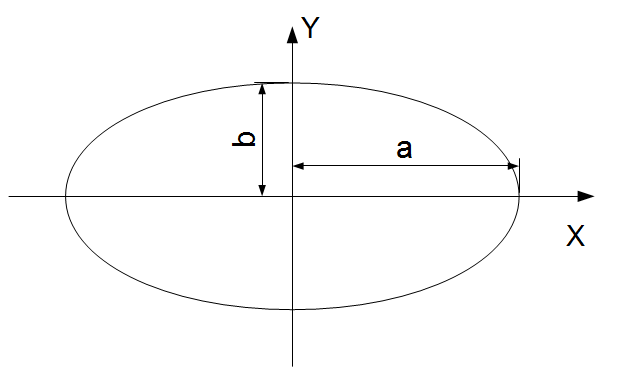
\includegraphics[scale=0.4]{Timo1.png}
  \caption{Visualización de la superficie de contacto cuando los radios de curvatura no son iguales entre si.}
  \label{fig:Timo1}
\end{figure} 


\begin{equation}
r_m=\sqrt[3]{\frac{3\pi}{8}\frac{P(k_1+k_2)}{\beta}}
\end{equation} 

Determinado el valor del radio promedio del contacto, los diámetros principales vienen definidos de acuerdo a una regla de proporcionalidad. Los valores m y n se definen por medio la excentricidad angular de la elipse de contacto
\begin{equation} 
a=m\cdot r_m
\end{equation} 
\begin{equation} 
b=n\cdot r_m
\end{equation} 

La excentricidad angular de la elipse de contacto, fue definida por Hertz según relaciones geométricas en función de la curvatura de las superficies. Conocidos los radios de curvaturas y expresados como $A$ y $B$, la excentricidad angular se determina mediante el cuadro \ref{tab:Hertzmn} descrita a continuación:

\begin{table}[!htbp]
\centering
\caption{Relación $m$ y $n$ respecto a al angulo $\theta$}

\begin{tabular}{ c | c c c c c c c  }

\label{tab:Hertzmn}

 $\theta$ & 90º & 80º & 70º & 60º & 50º & 40º & 30º \\ 
 \hline
 m & 1 & 1.128 & 1.285 & 1.486 & 1.754 & 2.136 & 2.731 \\ 
 n & 1 & 0.8927 & 0.8000 & 0.7171 & 0.6407 & 0.5673 & 0.4931 \\ 
\end{tabular} 

\end{table}


El ángulo $\theta$ que permite establecer la relación entre las curvaturas de las superficies con la proporción de los diámetros principales se calcula:

\begin{equation}
\theta=\arccos\left(\frac{B-A}{A+B}\right)
\end{equation}

Definidos $m$ y $n$, la distribución normal de presiones se conjuga como una superficie elipsoidal de ejes principales $a$, $b$ y  presión máxima  $q_0$:

\begin{equation}
\label{eq:NormHerz}
q=\frac{3}{2}\frac{P}{\pi a b}
\sqrt{1-\left(\frac{x}{a}\right)^2-
\left(\frac{y}{b}\right)^2}=q_0
\sqrt{1-\left(\frac{x}{a}\right)^2-
\left(\frac{y}{b}\right)^2}
\end{equation}

La metodología de \citet{Herz1881} es ampliamente utilizada para describir tanto los esfuerzos como los desplazamientos normales en el contacto entre dos cuerpos de superficies curvas. En el marco de los estudios de contacto mecánico rueda-riel, este método es la base de los sistemas de análisis dinámico de vehículos a la hora de estudiar la distribución de las presiones normales en la superficie de contacto simple.
 
A partir del modelo Hertz se plantean las primeras preguntas: ¿Si se conocen los desplazamiento normales del contacto mecánico, al igual que las presiones normales, es posible utilizar el modelo Hertz para evaluar las deformaciones en determinados puntos de una superficie para el caso concreto del contacto rueda-riel? ¿Se podrá definir una relación entre las deformaciones en la periferia de la rueda y las presiones normales en la zona de contacto?

La base de este modelo continúa con el estudio del comportamiento de las presiones tangenciales en el contacto rueda-riel, sin embargo todas las investigaciones posteriores mantienen el modelo de Hertz intacto.

\subsection{Inicio del modelado del contacto mecánico rueda-riel}
 
Debido al auge de los sistemas ferroviarios, se emprenden investigaciones sobre el fenómeno de rozamiento en contacto mecánico, en concreto para los sistemas rueda-riel. Para ello se introduce un nuevo término denominado como “fuga” o “deslizamiento”, como la separación entre las partículas de la rueda y el riel, tal como lo definen \citet{Carter1926}. Este modelo es considerado como la teoría exacta para las presiones tangenciales, sin considerar el deslizamiento distinto a la dirección de deslizamiento.

El estudio de las cargas tangenciales parte de la relación entre la fuerza tangencial y el límite de las cargas tangenciales representado por la ley de Coulomb para la fricción. Esta relación viene dada en función del deslizamiento expresado como:

  \begin{equation}
  \label{eq:Eq10}
  \frac{F_T}{\mu P}=-k\xi+\frac{1}{4}\cdot k^2 \xi \left|\xi \right|
  \end{equation}
  Donde:
  
  \begin{itemize}
  \item k es el coeficiente de deslizamiento de Carter $(4Rw/\nu a)$
  \item $\xi$ el deslizamiento longitudinal 
$2 \cdot (V_t-V_c)/(V_t+V_c)$
  \end{itemize}
 
 Suponiendo que no exista deslizamiento, los esfuerzos tangenciales y la presión entre las caras en el contacto rueda-riel ha de ser la misma en ambas superficies y la distribución de esfuerzos no se ve afectada por la tracción entre las superficies.
 
Considerando que el radio de la rueda es mayor que la circunferencia del contacto en sí, se puede asumir que el radio de la rueda es infinito. En la superficie de contacto se puede considerar que se trata de un medio finito elástico sujeto a un plano, donde existe una distribución de presiones y esfuerzos tangenciales debido a la tracción. Los esfuerzos y deformaciones debido a la presión son conocidas y no son discutidas más que para la transmisión de las fuerzas de tracción.
 
\begin{figure}[!htbp]
\centering
    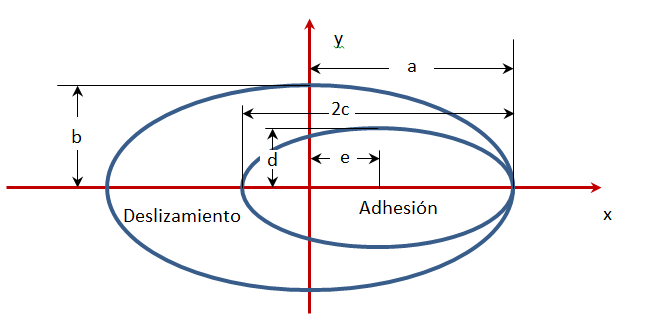
\includegraphics[scale=0.7]{Carter1.png}
  \caption{Descripción de la superficie de contacto bajo deslizamiento.}
  \label{fig:Carter1}
\end{figure}  
 
\bigskip  
  \par \hspace{2cm}
\begin{minipage}{8cm}
\begin{spacing}{0.5}
  Donde:
  \begin{itemize}
  \item $c$ y $d$ son las magnitudes de los ejes del área de adherencia.
 \item $e$ la distancia entre el centro de la elipse de Hertz respecto a centro de la elipse de
adhesión 
$ e=a-c$
  \end{itemize}
\end{spacing}
\end{minipage}
 
Primero se establece la existencia de dos áreas tal como se muestra en la figura \ref{fig:Carter1}. Un área de deslizamiento, donde la presión tangencial supera el límite de fricción estática dado por el roce entre la rueda y el riel y un área de adhesión, donde las deformaciones en la superficie de la rueda, no superan los límites de saturación por lo que no ocurre deslizamiento según el modelo de \citet{Carter1926}.

 
  La relación entre la geometría del área de adhesión y del deslizamiento con respecto a la fuerza de roce parte de la ecuación (\ref{eq:Eq10}) obteniendo:

 \begin{equation}
 \label{eq:Eq11}
 \frac{c}{a}=\frac{d}{b}=\sqrt[3]{1-\frac{F_T}{\mu P}}
 \end{equation}
  
  En este caso la presión tangencial en el área de adhesión viene expresada como:

  \begin{equation}
  \label{eq:Eq12}
  \tau (x,y)=
  \mu \cdot p_{n_{max}}\sqrt{
  1-
  \left(\frac{x}{a}\right)^2
  -\left(\frac{y}{b}\right)^2}
  +
  \mu \cdot \frac{c}{a} \cdot p_{n_{max}}\sqrt{
  1-
  \left(\frac{x-e}{c}\right)^2
  -\left(\frac{y}{d}\right)^2}
  \end{equation}
  
 El modelo de \citet{Carter1926} fue la motivación para una línea de investigación basada en este caso especial de contacto mecánico. El modelo analítico propuesto tiene la desventaja de sólo poder estudiar el caso bidimensional. Investigaciones realizadas en el campo del contacto rueda-riel como la de \citet{Kalker1971VSD} permitieron describir la distribución de presión tangencial para el problema tridimensional, describiendo las distribución de presión lateral y longitudinal, en este trabajo se considero el caso tridimensional, no obstante es necesario conocer las bases teóricas que llevaron a al análisis del contacto rueda-riel.

\subsection{La rugosidad y el contacto mecánico}
  
El estudio del contacto mecánico continuó; las investigaciones posteriores a \citet{Herz1881} se centraron en determinar el comportamiento del área de contacto. \citet{Herz1881} consideró las superficies de contacto lisas, sin ningún tipo de imperfecciones, esta consideración fue vista por \citet{Bowden07021939} como una limitación al modelo.

\citet{Bowden07021939} emprenden investigaciones sobre el comportamiento del área de contacto  con los resultados de Meyer (1898) que estableció una relación entre la resistencia eléctrica del metal y la presión que se ejercía.  
Años después, Auren (1903) y Browning (1906) presentaron resultados que demostraban lo contrario a las investigaciones de Meyer, lo cual llevó a concluir que podían presentar discordancias si no se limpiaba la superficie correctamente. Posteriormente se incluyen las observaciones de Blinder (1912) quien repite los ensayos realizado por los autores antes mencionados, arrojando que la conductancia eléctrica era menor a lo esperado y que por lo tanto el contacto era un área menor. Finalmente Holms (1922) señala que los resultados obtenidos se deben a dispersiones en la conductancia eléctrica, lo que sugiere que sobre la superficie plana existen varias áreas pequeñas de contacto.
  
\begin{figure}[!htbp]
\centering
    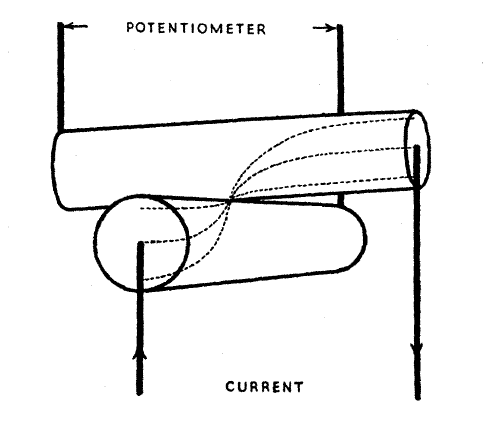
\includegraphics[scale=0.5]{Bowden1.png}
  \caption{Cilindros en contacto y el flujo de la corriente a través del punto de contacto. Fuente: \citet{Bowden07021939}}
  \label{fig:CilBownden}
\end{figure}   
  
\citet{Bowden07021939} en base a sus investigaciones bibliográficas deciden realizar experimentos con cilindros metálicos ubicados de manera transversal, con el fin de poder calcular el área contacto mediante la conductancia replicando los experimentos de Meyer (1898) como se muestra en la figura \ref{fig:CilBownden}. El resultado obtenido fueron descritos como variable en el tiempo ante cargas ligeras. Al aumentar la presión entre los cuerpos, aumentaba de manera considerable la conductancia eléctrica entre los cuerpos; al llevarse a cabo el experimento con cargas altas, se obtuvieron los resultados más estables, pero la dispersión se hacía presente ante ligeras vibraciones.

El comportamiento de la variaciones en la conductancia se definió  reproducible. En un principio se atribuyeron los resultados a la formación de óxido sobre la superficie. Al repetirse el experimento tomando en cuenta el movimiento entre los cuerpos, se verificó que se daba aún el comportamiento variante de la conductancia por lo que \citet{Bowden07021939} expresan la importancia de la fricción como factor influyente en las dimensiones de la superficie de contacto; adicionalmente especifica que el área
de contacto durante el movimiento presenta grandes fluctuaciones que sustentan la importancia de la fricción. Las fluctuaciones, de acuerdo con \citet{Bowden07021939}, dependerán de las propiedades de los materiales en contacto que determinan la velocidad con la que se forman y se rompen los contactos metálicos.
  
 Gracias al desarrollo tecnológico en el estudio de superficies, nace una nueva teoría en el contacto elástico considerando que la topografía de la superficie de estudio está directamente relacionada con el contacto superficial propuesta por \citet{Greenwood06121966}.  La investigación se inicia mediante un análisis estadístico del enlace; en primera instancia analizaron la distribución de irregularidades en la superficie, que limitan el contacto pleno entre los sólidos, asumiendo que el número de picos en contacto está directamente relacionado con el número de áreas en contacto.

\begin{equation}
\label{eq:Greenwood1}
prob(z>d)=\int_d^\infty \Phi(z) dz
\end{equation}

\par \hspace{1cm}
\begin{minipage}{10cm}
\begin{spacing}{0.5}
Donde los términos de la probabilidad de penetración de las rugosidades son:
\begin{itemize}
\item $z$ es la altura de la irregularidades.
\item $d$ es la distancia entre las dos superficies en contacto.
\item $\Phi(z)$ la distribución de las alturas de las irregularidades.
\end{itemize}
\end{spacing}
\end{minipage}


\begin{figure}[!htbp]
\centering
    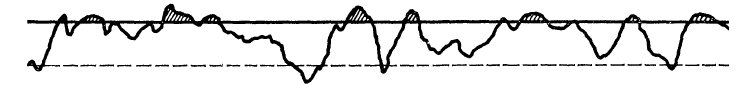
\includegraphics[scale=0.5]{Greenwood1.png}
  \caption{Perfil de rugosidades, donde se observa la región de penetración debido a la rugosidad y la zona donde el material se comporta como medio de elástico continuo.}
  \label{fig:Greenwood1}
\end{figure} 


  En segundo plano, a partir del número de áreas en contacto de acuerdo a la ecuación (\ref{eq:Greenwood2}) se puede determinar el área total de las superficies, como se describe en la ecuación (\ref{eq:Greenwood3}), que se encuentra realmente en contacto para luego poder determinar la conductancia y la carga aplicada en el experimento como se observa finalmente en las ecuaciones (\ref{eq:Greenwood4}) y (\ref{eq:Greenwood5}).

\begin{equation}
\label{eq:Greenwood2}
n=N \int_d^\infty \Phi(z) dz
\end{equation}

\par \hspace{1cm}
\begin{minipage}{10cm}
\begin{spacing}{0.5}
Donde:
\begin{itemize}
\item $n$ es la cantidades número de contactos.
\item $N$ es la cantidad de asperesas.
\end{itemize}
\end{spacing}
\end{minipage}

\begin{equation}
\label{eq:Greenwood3}
A=\delta A \cdot n=\pi N \beta \int_d^\infty (z-d)\Phi(z) dz
\end{equation}

El área de contacto viene definido a partir de \ref{eq:Greenwood3}:

\par \hspace{1cm}
\begin{minipage}{10cm}
\begin{spacing}{0.5}
\begin{itemize}
\item $A$ es el área total en contacto.
\item $\delta A$ es el área de cada punto de contacto.
\item $\beta$ la sumatoria de las curvaturas de la superficies, basado en la teoría de Hertz.
\end{itemize}
\end{spacing}
\end{minipage}

Siguiendo bajo el modelo de contacto mecánico de \citet{Herz1881} la carga total entre las dos superficies viene dado por la integración de la distribuciones de presiones de cada puntos.

\begin{equation}
\label{eq:Greenwood4}
P=\frac{4}{3}\pi N (k_1+k_2) \sqrt{\beta} \int_d^\infty (z-d)^{3/2}\Phi(z) dz
\end{equation}

\par \hspace{1cm}
\begin{minipage}{10cm}
\begin{spacing}{0.5}
\begin{itemize}
\item $P$ representa la carga aplicada total.
\item $k_n$ las constantes elásticas de Hertz.
\end{itemize}
\end{spacing}
\end{minipage}

Ya que la conducción eléctrica depende del área contacto y esta a su vez depende de la carga, a partir de \ref{eq:Greenwood4}, se obtiene:

\begin{equation}
\label{eq:Greenwood5}
G=\frac{2N (k_1+k_2) \sqrt{\beta}}{\rho}
 \int_d^\infty \sqrt{(z-d)}\Phi(z) dz
\end{equation}

\par \hspace{1cm}
\begin{minipage}{10cm}
\begin{spacing}{0.5}
Donde:
\begin{itemize}
\item $G$ la conductancia del contacto.
\item $\rho$ la impedancia del material.
\end{itemize}
\end{spacing}
\end{minipage}

Se debe añadir que \citet{Greenwood06121966}, definen un criterio para determinar un contacto elástico o plástico, denominado índice de plasticidad definido en la ecuación (\ref{eq:Greenwood6}). Este índice establece los rangos de dureza elástica y dureza real. Si el índice de plasticidad es bajo, es poco probable que el modo de deformación cambie por efecto de la carga, por lo cual es incorrecto alegar que si un cuerpo no sufre deformaciones permanentes en su superficie, éste las sufrirá aumentando la carga.

\begin{equation}
\label{eq:Greenwood6}
\Psi=\frac{(k_1+k_2)\cdot h'}{Sy}
\end{equation}

\par \hspace{2cm}
\begin{minipage}{8cm}
\begin{spacing}{0.5}
Donde:
\begin{itemize}
\item $\Psi$ es el índice de plasticidad.
\item $h'$ el promedio de la rugosidad.
\item $Sy$ es la resistencia del material.
\end{itemize}
\end{spacing}
\end{minipage}

  Las respuestas encontradas por \citet{Greenwood06121966}, determinaron la diferencia entre el área nominal de contacto (ejercida por una carga nominal) y el área de contacto real dado por la distribución de cargas en los micro-contactos en las superficies; la comparación de los resultados determinó que la separación entre los cuerpos obtuvieron una desviación estándar de 1 o 2; según lo expresaron los autores, la separación real entre las superficies, para amplios rangos de cargas, son semejantes a la separación promedio estimada. 

 
\subsection{Modelado tridimensional de contacto rueda-riel} 
 
La relación entre las fuerzas tangenciales y el límite de roce estático entre las superficies de la rueda y el riel respecto al deslizamiento propuesto por \citet{Carter1926}, fue simplificada por Pater y Johnson resultando en:

  \begin{equation}
  \label{eq:Eq13}
  \frac{F_T}{\mu P}=-k\xi
  \end{equation}

Esta simplificación permitió la creación de la teoría lineal de contacto rueda-riel para establecer un modelo basado en la
aproximación de Winkler, donde los enlaces elásticos en la superficie de contacto son sustituidos por resortes equivalentes de constante elástica $L$. Este modelo se denomina teoría simplificada de \citet{Kalker1971VSD} y permite el estudio tridimensional de las presiones presentes en el contacto rueda riel. Para ello es necesario definir dos nuevos deslizamiento, denominados deslizamiento lateral y rotacional.

Una de las limitaciones del modelo de Carter, es la dificultad que parte de estudiar el contacto para el caso tridimensional. La linealidad del modelo de \citet{Kalker1971VSD} permite considerar los deslizamientos en distintas direcciones, en especial, los deslizamientos longitudinales, lateral y rotacionales.

La determinación del deslizamiento longitudinal, lateral y rotacional ($\xi$, $\eta$ y $\phi$) viene dada por la ubicación o posición de la rueda respecto al conjunto del eje y ruedas como cuerpo rígido. La geometría de la rueda juega un rol importante en la determinación de los deslizamientos longitudinales:

\begin{equation}
\label{DezlLong}
\xi=\frac{V-r\omega}{0.5(V-r\omega)}=-\frac{\Delta r}{r_o}=-\gamma\frac{y}{r_o}
\end{equation}

\par \hspace{1cm}
\begin{minipage}{10cm}
\begin{spacing}{0.5}
Donde:
\begin{itemize}
\item $\omega$ es la velocidad rotacional de la rueda.
\item $r$ el radio de la rueda en el punto de contacto.
\item $V$ la velocidad del eje.
\item $\gamma$ es la conicidad de la rueda.
\item $r_o$ es el radio de la rueda en la posición ideal.
\item $y$ el movimiento lateral de la eje.
\end{itemize}
\end{spacing}
\end{minipage}

El deslizamiento lateral, depende del ángulo que forma  la rueda respecto a su dirección de traslación:

\begin{equation}
\phi=\alpha
\end{equation}

\par \hspace{1cm}
\begin{minipage}{10cm}
\begin{spacing}{0.5}
Donde $\alpha$ es el ángulo que forma la dirección de traslación respecto a la velocidad de rotación.
\end{spacing}
\end{minipage}

El deslizamiento rotacional en cambio depende de la geometria de la rueda en el punto de contacto y la conicidad de la rueda.

\begin{equation}
\eta=\frac{\sin(\gamma)}{r}
\end{equation}

Conocidos los deslizamientos, y recordando la linealidad de la Teoría Simplificada, se puede establecer una relación directamente proporcional de las cargas en las coordenadas ($x$,$y$) obteniendo:

\begin{equation}
\label{eq:Kalkerlong}
F_x=-Gabc_{11}\xi
\end{equation}
\begin{equation}
\label{eq:Kalkerlat}
F_{y_{lat}}=-Gabc_{22}\eta
\end{equation}
\begin{equation}
\label{eq:Kalkerrot}
F_{y_{rot}}=-Gabc_{23} \cdot \sqrt{ab} \phi
\end{equation}

Es a partir del conocimiento de las fuerzas laterales y longitudinales que se estableció un modelo basado la solución de Winkler (suponer un cuerpo elástico como un conjunto de resortes conectados a puntos rígidos del cuerpo).  Para ello, se asume que cada resorte en el momento del contacto mecánico tiene una constante $L_m$ donde $m$ es la dirección del deslizamiento.

\begin{equation}
\label{eq:L1}
L_\xi=\frac{8a}{3C_{11}G}
\end{equation}

\begin{equation}
\label{eq:L2}
L_\eta=\frac{8a}{3C_{22}G}
\end{equation}

\begin{equation}
\label{eq:L3}
L_\phi=\frac{8a\sqrt{a/b}}{4C_{23}G}
\end{equation}

Conocidos los valores de $L_m$ mediante (\ref{eq:L1}),(\ref{eq:L2}) y (\ref{eq:L3}), se puede obtener un valor de $L$ general, proyectando las componentes de cada constante a la dirección del deslizamiento, de modo que se transforma el problema tridimensional, a un problema bidimencional:

\begin{equation}
\label{eq:Lgen}
L=\frac{
\left(
|\xi |L_\xi + |\eta |L_\eta + \sqrt{ab}|\xi |L_\phi
\right)
}
{
\sqrt{
\xi ^2+\eta ^2+ ab \xi^2
}
}
\end{equation}

Conocido $L$ como la constante elástica por unidad de presión tangencial para las deformaciones normales colineales con el movimiento de la rueda. Se puede abordar el problema del contacto mecánico rueda riel mediante las deformaciones de la rueda y el riel:

\begin{equation}
\label{eq=Defor}
u_x=L\cdot \tau
\end{equation}

El concepto de domo de saturación, o la máxima presión tangencial debido a la presión normal, establece los limites del desplazamiento de las partículas en dirección del movimiento del eje:

\begin{equation}
\label{eq=DeforMax}
u_{max}=L\cdot \mu p_n
\end{equation}

Por último, si se estudia la relación entre el deslizamiento rígido y el deslizamiento elástico, se hacen presentes las deformaciones en la superficie del contacto obteniendo la base de la teoría de Kalker:

\begin{equation}
\label{DifSol}
\frac{du_x}{dx}=s(x)-w(x)
\end{equation}

\par \hspace{1cm}
\begin{minipage}{10cm}
\begin{spacing}{0.5}
Donde:
\begin{itemize}
\item $\frac{du_x}{dx}$ las deformaciones en la dirección de traslación de la rueda.
\item $w(x)$ es el deslizamiento rígido de la rueda.
\item $s(x)$ el deslizamiento elástico de la rueda.
\end{itemize}
\end{spacing}
\end{minipage}

La ecuación (\ref{DifSol}) tiene solución analítica al derivar el domo de saturación, donde $s(x)$ es diferente de cero cuando $w(x)>\frac{du_{max}}{dx}$. Sin embargo Kalker propuso una solución mediante diferencias finitas utilizando el método de euler, esto se debe a que la ecuación (\ref{DifSol}) solo considera las deformaciones en la dirección de traslación, pudiendo aceptar otros modelos de contacto mecánico normal, diferentes a la geometría de Hertz. La solución entonces es:

\begin{equation}
\label{EulerSol}
u_i=u_{i-1}+\delta x\cdot s_i-\delta x\cdot w(x_i)
\end{equation}

\par \hspace{2cm}
\begin{minipage}{8cm}
\begin{spacing}{0.5}
Donde $\delta x$ es el espesor de grilla elegido para el cálculo mediante diferencias finitas. 
\end{spacing}
\end{minipage}

El algoritmo inicia con $u_0=0$ y $s_0=0$ y en $x_0=-a$ y evalúa en cada iteración si $u_i>u_{max}$ se define: $u_i=u_{max}$ y $s_i=\frac{u_i-u_{i-1}}{\delta x}+w_i$.

La solución de Kalker es ampliamente utilizada en el estudio del contacto rueda riel por su rapidez y sencillez de uso, pero el modelo también genera dudas: ¿Puede el modelo Kalker adaptarse para estudiar la rugosidad y el efecto en las presiones tangenciales? ¿De qué manera las presiones tangenciales influyen en las deformaciones en la superficie de la rueda?

El modelo de Kalker es efectivo cuando los deslizamiento son cercanos a los límites de la fricción pura bajo las consideraciones lineales. El modelo de Shen-Hedrick-Elkins permite definir con mejor precisión el comportamiento no lineal del contacto mecánico rueda-riel sometido a deslizamiento, esto con el fin de determinar las cargas en la dirección longitudinal y lateral.

El modelo de Shen-Hedrick-Elkins parte del modelo de Kalker para el cálculo de cargas en la dirección del movimiento y la dirección lateral (\ref{eq:Kalkerlong}), (\ref{eq:Kalkerlat}) y (\ref{eq:Kalkerrot}).

\begin{displaymath}
F_x=-Gabc_{11}\xi
\end{displaymath}
\begin{displaymath}
F_y=-Gabc_{22}\eta - Gabc_{23} \cdot \sqrt{ab} \phi
\end{displaymath}

El módulo de la suma vectorial de estas dos fuerzas viene dada por:

\begin{equation}
F_T=\sqrt{F_x^2+F_y^2}
\end{equation}

El modelo por tanto se logra aproximando la relación entre carga tangencial y carga máxima por un polinomio de tercer grado:

\begin{equation}
F'_T=
\begin{cases} 
\begin{matrix} \mu N 
\left[ 
\left(
\frac{F_T}{\mu N}
\right)
-\frac{1}{3}
\left(
\frac{F_T}{\mu N}
\right)^2 
+\frac{1}{27}
\left(
\frac{F_T}{\mu N}
\right)^3 
\right]
 & F_T\le 3\mu N \\\mu N & F_T> 3\mu N 
\end{matrix} 
\end{cases}
\end{equation}

\par \hspace{2cm}
\begin{minipage}{8cm}
\begin{spacing}{0.5}
Donde $F'_T$ es el módulo de la carga tangencial aplicada corregido según el modelo de Shen-Hedrick-Elkins.
\end{spacing}
\end{minipage}

Finalmente para calcular las fuerzas tangenciales en la dirección longitudinal y lateral se obtiene:

\begin{eqnarray}
F'_x=F'_T\frac{F_x}{F_T}\\
F'_y=F'_T\frac{F_y}{F_T}
\end{eqnarray}

Una de las características del modelo radica en que el momento por rotación no se toma en cuenta. Este resultado es más preciso que el modelo de Kalker fuera del rango lineal pero no es recomendable para altos valores de deslizamiento tal como lo menciona \citet{springerlink:10.1007/s11044-007-9094-y}.

Ante la necesidad de un método fiable y continuo para parámetros de deslizamiento altos y que además considere el momento rotacional, se estableció un modelo basado en una solución estandarizada de la totalidad de fuerzas tangenciales, conocido como la formulación de \citet{Polach1999}.

El modelo \citet{Polach1999} parte de una geometría conocida de presiones tangenciales siendo el gradiente de presiones tangenciales, en la zona de adhesión, lineal respecto la dirección de movimiento, tal como se muestra en la figura \ref{fig:Polach}.

\begin{figure}[!htbp]
\centering
    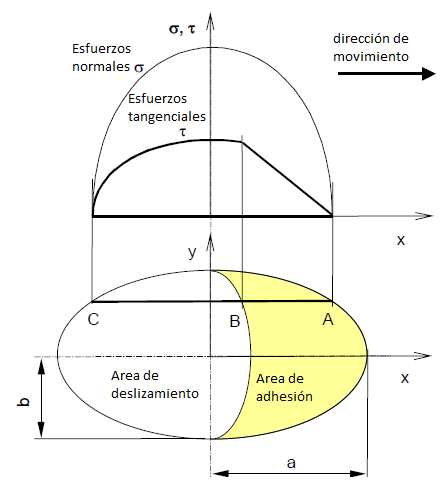
\includegraphics[scale=0.7]{Polach1.png}
  \caption{Geometría de la distribución de esfuerzos; \citet{Polach1999}.}
  \label{fig:Polach}
\end{figure}  

La integración de esta geometría fue calculada por Freibauer como menciona \citet{Polach1999}. Para ello es necesario transformar el elipsoide de contacto es una esfera de radio a.

\begin{equation}
y'=\frac{a}{b}\cdot y, \; \tau'=\frac{a}{\tau_0}\cdot \tau
\end{equation}

\par \hspace{1cm}
\begin{minipage}{10cm}
\begin{spacing}{0.5}
Donde:
\begin{itemize}
\item  $y'$ es la transformación a escala de las dimensiones en el eje $y$.
\item $a$ y $b$ es la magnitud de las diámetros principales de la superficie de contacto.
\item $\tau$ la presión tangencial.
\item $\tau_O$ la presión tangencial máxima.
\item $\tau'$ la presión tangencial máxima a escala.
\end{itemize}
\end{spacing}
\end{minipage}

Definiendo la nueva geometría de la presión tangencial de contacto a escala, la integración de la presión tangencial da como resultado la carga tangencial aplicada.

\begin{equation}
F_T=\iint \tau dx dy=\tau_0 \frac{b}{a^2} \iint \tau' dx dy'
\end{equation}

Dando como resultado:

\begin{equation}
\label{eq:Polach1}
F_T=-\tau_0\frac{b}{a^3}\frac{4}{3}a^3
\left(
\frac{\epsilon}{1+\epsilon^2}+\arctan{\epsilon}
\right)
\end{equation}

\par \hspace{2cm}
\begin{minipage}{8cm}
\begin{spacing}{0.5}
Donde $\epsilon$ es el gradiente de los esfuerzos tangenciales en el área de adhesión y está definido como:
\end{spacing}
\end{minipage}

\begin{equation}
\epsilon=\frac{2}{3}\frac{C\pi a^2 b}{\mu N}\upsilon
\end{equation}

Para lo cual, la constante de proporcionalidad $C$  viene dada por la elasticidad de los cuerpos y $\upsilon=\sqrt{\xi^2+\upsilon_y^2}$ el deslizamiento total. La ecuación (\ref{eq:Polach1}) puede ser simplificada mediante la relación $\tau_0=\mu P_{n_{max}}$, de esta manera se obtiene:

\begin{equation}
F_T=-\frac{2\mu N}{\pi}
\left(
\frac{\epsilon}{1+\epsilon^2}+\arctan{\epsilon}
\right) 
\end{equation}

Desde este punto las cargas longitudinales pueden ser calculadas considerando el deslizamiento longitudinal $\xi$ como:

\begin{equation}
F_x=F_T\frac{\xi}{\upsilon}
\end{equation}

Para determinar la magnitud de las cargas laterales $F_y$ hay que descomponer esta carga por las componentes del deslizamiento lateral y rotacional, las cuales tendrán la nomenclatura  $F_{y\eta}$ y $F_{y\phi}$. El cálculo parte desde la determinación del deslizamiento lateral total:

\begin{equation}
\upsilon_y=
\begin{cases} 
\begin{matrix}
\eta+\phi \cdot a & si \; |\eta+\phi \cdot a|>|\eta|
\\
\eta & si \; |\eta+\phi \cdot a|\le|\eta|
\end{matrix}
\end{cases}
\end{equation}

Para el caso de las cargas laterales motivado a la inclinación de la rueda respecto al riel $F_{y\eta}$, el cálculo es el mismo que las cargas longitudinales $F_x$, sin embargo las cargas laterales motivados al giro de la rueda respecto a la normal de la superficie de contacto $F_{y\phi}$ es un valor especifico calculado por la misma metodología implementada en la ecuación (\ref{eq:Polach1}) obteniendo:

\begin{equation}
F_{y\phi}=-\frac{9}{16}a\mu N K_M \left[1+6.3\left(1-e^\frac{a}{b}\right)\right]\frac{\phi}{\upsilon}
\end{equation}

Donde $K_M$ se define:

\begin{equation}
K_M=|\epsilon |
\left(\frac{\delta^3}{3}+\frac{\delta^2}{2}+\frac{1}{6}\right)-\frac{1}{3}\sqrt{(1-\delta^2)^3}
\end{equation}

Y $\delta$ como:

\begin{equation}
\delta=\frac{\epsilon_s^2-1}{\epsilon_s^2+1}
\end{equation}

Donde la modificación de $\epsilon_s$ es descrita como:
\begin{equation}
\epsilon_s=
\frac{2}{3}
\frac{C\pi a^2 b}{\mu N}
\frac{ S_{yC}}{ \left[1+6.3\left(1-e^{-\frac{a}{b}}\right)\right]}
\end{equation}


La determinación de la constante $C$ de elasticidad, puede ser calculada mediante pruebas experimentales o relacionándola con la teoría de Kalker evaluándola en $\epsilon \rightarrow 0$ de modo que $\epsilon$ y $\epsilon_s$ se pueden definir gracias a las constantes de kalker como:

\begin{equation}
\epsilon=\frac{1}{4}\frac{G\pi a b c_{jj}}{\mu N}\upsilon
\end{equation}
Donde el la constante geométrica viene dado $c_{jj}=\sqrt{
\left(c_{11}\frac{\xi}{\upsilon}\right)^2
+
\left(c_{22}\frac{\eta}{\upsilon}\right)^2
}$ mientras que $\epsilon_s$:
\begin{equation}
\epsilon_s=\frac{8}{3}\frac{G b \sqrt{a\cdot b}}{\mu N}\frac{ c_{23}\upsilon_y}{ \left[1+6.3\left(1-e^\frac{a}{b}\right)\right]}
\end{equation}

Las constantes de elasticidad $c_{11}$, $c_{22}$ y $c_{23}$ fueron definidas por \citet{Kalker1991243}.

El propósito de la propuesta \citet{Polach1999} fue obtener un algoritmo para calcular rápidamente las cargas laterales y longitudinales. siendo lo más preciso posible cuando el modelo lineal no determina con precisión el comportamiento de las cargan tangenciales.

De esta manera se hace una revisión de los cuatro métodos implementados para el estudio del contacto rueda riel, siendo \citet{Kalker1971VSD} y \citet{Polach1999} los más utilizados comercialmente.

\end{document}
